\documentclass[paper.tex]{subfiles}

\usepackage{tikz}
\usepackage{amsmath}
\usepackage{graphicx}
\usepackage{tabularx}
\usepackage{multicol}
\usepackage{algpseudocode}
\usepackage{algorithm}

% Add vertical spacing to tables
\renewcommand{\arraystretch}{1.4}

% Begin Document
\begin{document}

\section{Background}

The Minimum Dominating Set of a Graph is defined as the set of vertices for which each vertex or one of its neighbors is in the set.
Consider the graph in Figure 1.

\begin{figure}
    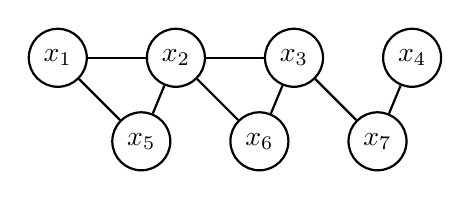
\begin{tikzpicture}[node distance={15mm}, thick, main/.style = {draw, circle}] 
        \node[main] (1) {$x_1$};  
        \node[main] (2) [right of = 1] {$x_2$};  
        \node[main] (3) [right of = 2] {$x_3$};  
        \node[main] (4) [right of = 3] {$x_4$};
        \node[main] (5) [below right of = 1] {$x_5$};
        \node[main] (6) [below right of = 2] {$x_6$};
        \node[main] (7) [below right of = 3] {$x_7$};  
        \draw (1) -- (5);
        \draw (1) -- (2);
        \draw (2) -- (3);
        \draw (2) -- (5);
        \draw (2) -- (6);
        \draw (3) -- (6);
        \draw (3) -- (7);
        \draw (4) -- (7);  
    \end{tikzpicture}
    \caption{Graph with 7 Vertices}
\end{figure}

\end{document}